\documentclass[a4paper,12pt]{article}

% Paquetes básicos
\usepackage[utf8]{inputenc}
\usepackage[T1]{fontenc}
\usepackage[spanish]{babel}
\usepackage{graphicx}
\usepackage{xcolor}
\usepackage{lipsum}
\usepackage{geometry}
\geometry{top=3cm, bottom=3cm, left=2.5cm, right=2.5cm}

% Paquetes para diseño
\usepackage{titlesec}
\usepackage{fancyhdr}
\usepackage{amsmath}
\usepackage{amssymb}
\usepackage{hyperref}
\usepackage{pdfpages}
\usepackage{markdown}

% Paquetes para el entorno lstlisting
\usepackage{listings}
\usepackage{inconsolata}

% Paquete para fondo
\usepackage{background}

% Configuración de lstlisting
\lstset{
    language=Python,
    basicstyle=\ttfamily\small,
    keywordstyle=\color{blue}\bfseries,
    stringstyle=\color{teal},
    commentstyle=\color{gray}\itshape,
    numbers=left,
    numberstyle=\tiny\color{gray},
    backgroundcolor=\color{black!5},
    frame=single,
    rulecolor=\color{black!50},
    breaklines=true,
    captionpos=b,
    showstringspaces=false
}

% Configuración de título
\titleformat{\section}{\normalfont\Large\bfseries}{\thesection}{1em}{}

% Información del documento
\title{
    \vspace{-2cm}
    
\includegraphics[width=0.3\textwidth]{../images/fccee.jpg} \\ % Cambia el logo si es necesario
    \LARGE Ingeniería Informática + ADE\\
    \large Universidad de Granada (UGR)\\[1cm]
}
\author{\textbf{Autor:} Ismael Sallami Moreno}
\date{\textbf{Asignatura:} Contabilidad Financiera I}

% Configuración del fondo
\backgroundsetup{
    scale=1,
    color=black,
    opacity=0.2,
    angle=0,
    position=current page.south,
    vshift=0pt,
    hshift=0pt,
    contents={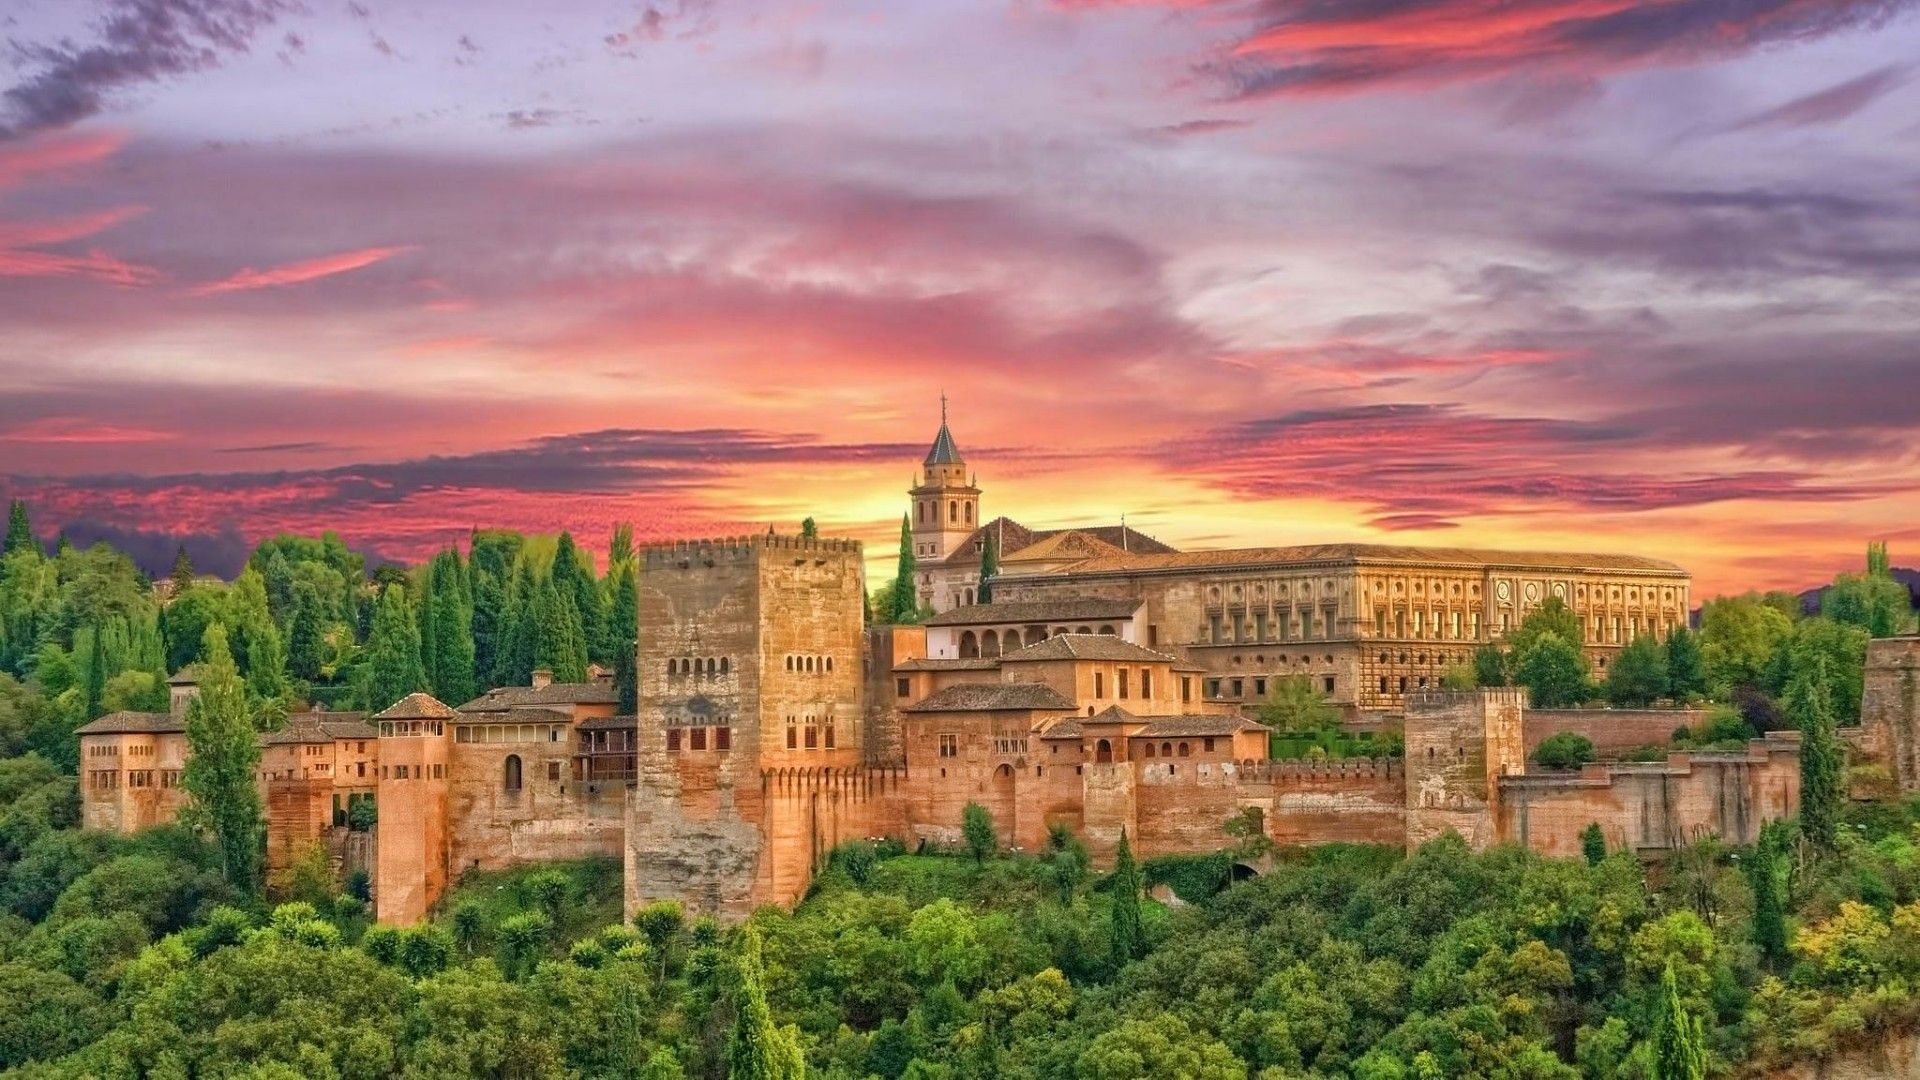
\includegraphics[width=\paperwidth,height=\paperheight,keepaspectratio]{../images/granada.jpg}}
}

% Inicio del documento
\begin{document}

% Portada
\maketitle
\thispagestyle{empty}

\begin{center}
    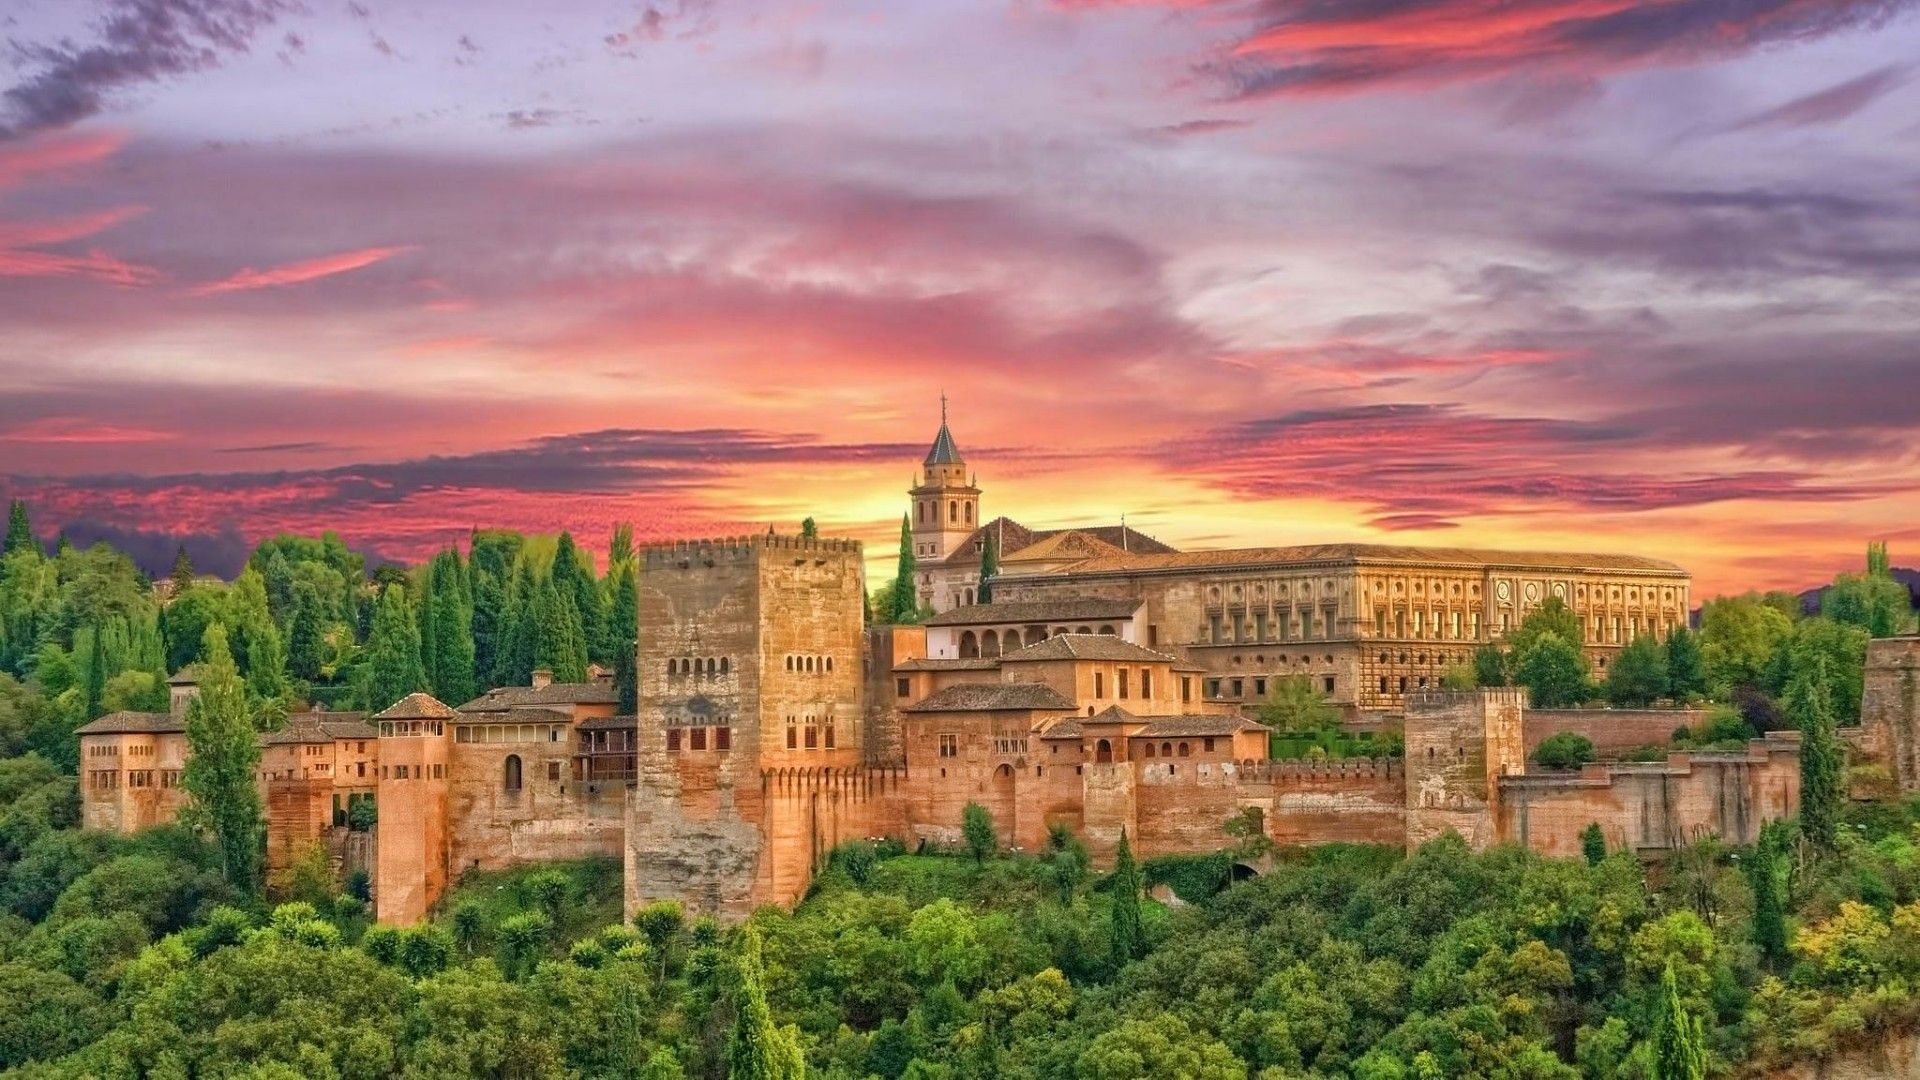
\includegraphics[width=\textwidth,height=0.4\textheight,keepaspectratio]{../images/granada.jpg} \\ % Añade tu imagen de fondo
    \vfill
\end{center}

\newpage

% Índice (opcional)
\tableofcontents
\newpage

\section{Libro de Prácticas}


\includepdf[pages=-]{Libro.pdf}

\section{Resoluciones}

\subsection{Tema 2}
\includepdf[pages=-]{../Tema2/T2.pdf}
\subsection{Tema 3}

\includepdf[pages=-]{../Tema3/T3.pdf}
\subsection{Tema 4}
% \section*{Ejercicio Propuesto 8}

La sociedad FAITH, S.A. realiza las siguientes operaciones durante el mes de diciembre:

\begin{itemize}
    \item Compra mercaderías en el Reino Unido por un importe de 15.000 £ a un tipo de cambio de 1 £/1,4 €. El pago se realizará dentro de tres meses sin interés contractual.
    \item Vende mercaderías en EEUU por un importe de 20.000 \$ a un tipo de cambio de 0,70 €/\$. El cobro se hará efectivo dentro de 6 meses sin interés contractual.
    \item Compra dólares por valor de 15.000 € para poder realizar pagos en esta divisa, siendo el tipo de cambio en ese momento de 0,75 €/\$.
    \item A 31 de diciembre los tipos de cambio son: 1,6 €/£ y 0,80 €/\$.
\end{itemize}

\subsection*{1. Contabilice la compra en el Reino Unido}

\begin{table}[h!]
\centering
\begin{tabular}{|c|l|c|}
\hline
\textbf{DEBE} & \textbf{CUENTA} & \textbf{HABER} \\ \hline
              & (4004) Proveedores moneda extranjera & 15.000 * 1,4 = 21.000 € \\ \hline
21.000 €      & (600) Compra de mercaderías & \\ \hline
\end{tabular}
\end{table}

\subsection*{2. Contabilice la venta en EE.UU.}

\begin{table}[h!]
\centering
\begin{tabular}{|c|l|c|}
\hline
\textbf{DEBE} & \textbf{CUENTA} & \textbf{HABER} \\ \hline
              & (700) Venta de mercaderías & 20.000 * 0,7 = 14.000 € \\ \hline
14.000 €      & (4304) Cliente en moneda extranjera & \\ \hline
\end{tabular}
\end{table}

\subsection*{3. Contabilice la compra de dólares}

\begin{table}[h!]
\centering
\begin{tabular}{|c|l|c|}
\hline
\textbf{DEBE} & \textbf{CUENTA} & \textbf{HABER} \\ \hline
              & (572) Bancos & 15.000 € \\ \hline
15.000 €      & (573) Banco en moneda extranjera & \\ \hline
\end{tabular}
\end{table}

\subsection*{4. Regularización de las diferentes monedas a 31 de diciembre}

\begin{table}[h!]
\centering
\begin{tabular}{|c|l|c|}
\hline
\textbf{DEBE} & \textbf{CUENTA} & \textbf{HABER} \\ \hline
3.000 €       & (668) Diferencias negativas de cambio (pérdidas) & \\ \hline
              & (4004) Proveedores moneda extranjera & 3.000 € \\ \hline
2.000 €       & (768) Diferencias positivas de cambio (ganancias) & \\ \hline
              & (4304) Clientes en moneda extranjera & 2.000 € \\ \hline
\end{tabular}
\end{table}

\textbf{Cálculos:}
\begin{itemize}
    \item A 1 de diciembre: 15.000 £ * 1,4 €/£ = 21.000 €.
    \item A 31 de diciembre: 15.000 £ * 1,6 €/£ = 24.000 €. Diferencia negativa: 3.000 €.
    \item A 1 de diciembre: 20.000 \$ * 0,7 €/\$ = 14.000 €.
    \item A 31 de diciembre: 20.000 \$ * 0,8 €/\$ = 16.000 €. Diferencia positiva: 2.000 €.
\end{itemize}

\subsection*{5. Ajuste de la moneda extranjera a 31/12/2023}

\begin{table}[h!]
\centering
\begin{tabular}{|c|l|c|}
\hline
\textbf{DEBE} & \textbf{CUENTA} & \textbf{HABER} \\ \hline
1.500 €       & (668) Diferencias negativas de cambio & \\ \hline
              & (4004) Proveedores moneda extranjera & 1.500 € \\ \hline
\end{tabular}
\end{table}

\textbf{Cálculos:}
\begin{itemize}
    \item 15.000 \$ * 1,2 €/\$ = 18.000 € (1 de septiembre).
    \item 15.000 \$ * 1,3 €/\$ = 19.500 € (31 de diciembre).
    \item Diferencia negativa: 1.500 €.
\end{itemize}

\subsection*{6. Ajuste del contrato de limpieza}

\begin{table}[h!]
\centering
\begin{tabular}{|c|l|c|}
\hline
\textbf{DEBE} & \textbf{CUENTA} & \textbf{HABER} \\ \hline
7.562,50 €    & (480) Gastos anticipados & \\ \hline
              & (625) Servicios de profesionales independientes & 7.562,50 € \\ \hline
\end{tabular}
\end{table}

\textbf{Cálculos:}
\begin{itemize}
    \item Contrato: 9.982,50 € (IVA incluido).
    \item Sin IVA: 9.982,50 / 1,21 = 8.250 €.
    \item Servicio de 6 meses, devengados 5,5 meses hasta el 31 de diciembre.
    \item 8.250 € / 6 * 5,5 = 7.562,50 €.
\end{itemize}

\section*{Ejercicio Propuesto 8 del Libro Nuevo (2024-2025)}

La empresa Beta S.A. entregó un anticipo el 15 de septiembre de 2022 a uno de sus empleados por 20.000 €. El 31 de diciembre de 2022 esta empresa contabiliza la nómina de los empleados que corresponden a 5 trabajadores con las mismas remuneraciones.

El sueldo bruto de los empleados fue de 130.000 €. Las cuotas de Seguridad Social fueron 10.000 € a cargo de los empleados y 40.000 € a cargo de la empresa. Las retenciones por IRPF supusieron el 15%. Por problemas de liquidez, Beta S.A. solo pudo pagar la nómina de dos empleados, entre los que estaba el que había dado un anticipo, el cual fue descontado completamente en su nómina. La nómina de los 3 empleados restantes quedó pendiente de pago.

Por otra parte, esta empresa Beta adquirió el 01/09/2023 a una empresa estadounidense mercaderías por valor actual de 30.000 €, cuando la cotización era de 1,2 €/\$.(sin IVA) (operación exenta de IVA). El pago de la mitad de esta compra se aplazó 12 meses acordando un interés contractual efectivo compuesto anual del 5\%. La cotización a 31/12/2023 era 1,5 €/\$.

Además, la empresa Beta formalizó un contrato para la limpieza de sus instalaciones con la empresa Sigma S.L. El contrato se formalizó el 01/09/2023 firmando una letra por importe de 9.982,5 € (IVA incluido del 21%) y vencimiento a 3 meses. El contrato incluía la prestación del servicio de limpieza 6 meses, iniciándose el servicio el 15/12/2023.

\subsection*{SE PIDE:}
Teniendo en cuenta la información anterior contabilice:

\subsubsection*{(a) Devengo de la nómina y seguridad social de la empresa a 31/12/2022}

\begin{table}[h!]
\centering
\begin{tabular}{|c|l|c|}
\hline
\textbf{DEBE} & \textbf{CUENTA} & \textbf{HABER} \\ \hline
130.000 €     & (640) Sueldos y Salarios & \\ \hline
40.000 €      & (642) Seguridad Social a cargo de la empresa & \\ \hline
              & (476) Organismos de la Seguridad Social Acreedores & 50.000 € \\ \hline
              & (4751) Hacienda Pública, retenciones y pagos a cuenta & 19.500 € \\ \hline
              & (460) Anticipos de remuneraciones & 20.000 € \\ \hline
              & (572) Bancos & 20.200 € \\ \hline
              & (465) Remuneraciones pendientes de pago & 60.300 € \\ \hline
\end{tabular}
\end{table}

\textbf{Cálculos:}
\begin{itemize}
    \item Sueldo bruto: 130.000 €
    \item Seguridad Social a cargo de los empleados: 10.000 €
    \item Seguridad Social a cargo de la empresa: 40.000 €
    \item Retenciones por IRPF: 130.000 € * 0.15 = 19.500 €
    \item Anticipo descontado: 20.000 €
    \item Pago de nómina de dos empleados: 26.000 € * 2 - 2.000 € * 2 - 3.900 € * 2 = 40.200 €
    \item Pago de nómina de un empleado con anticipo: 26.000 € - 2.000 € - 3.900 € - 20.000 € = 100 €
    \item Total pagado: 40.200 € + 100 € = 40.300 €
    \item Remuneraciones pendientes de pago: 130.000 € - 40.300 € = 89.700 €
\end{itemize}

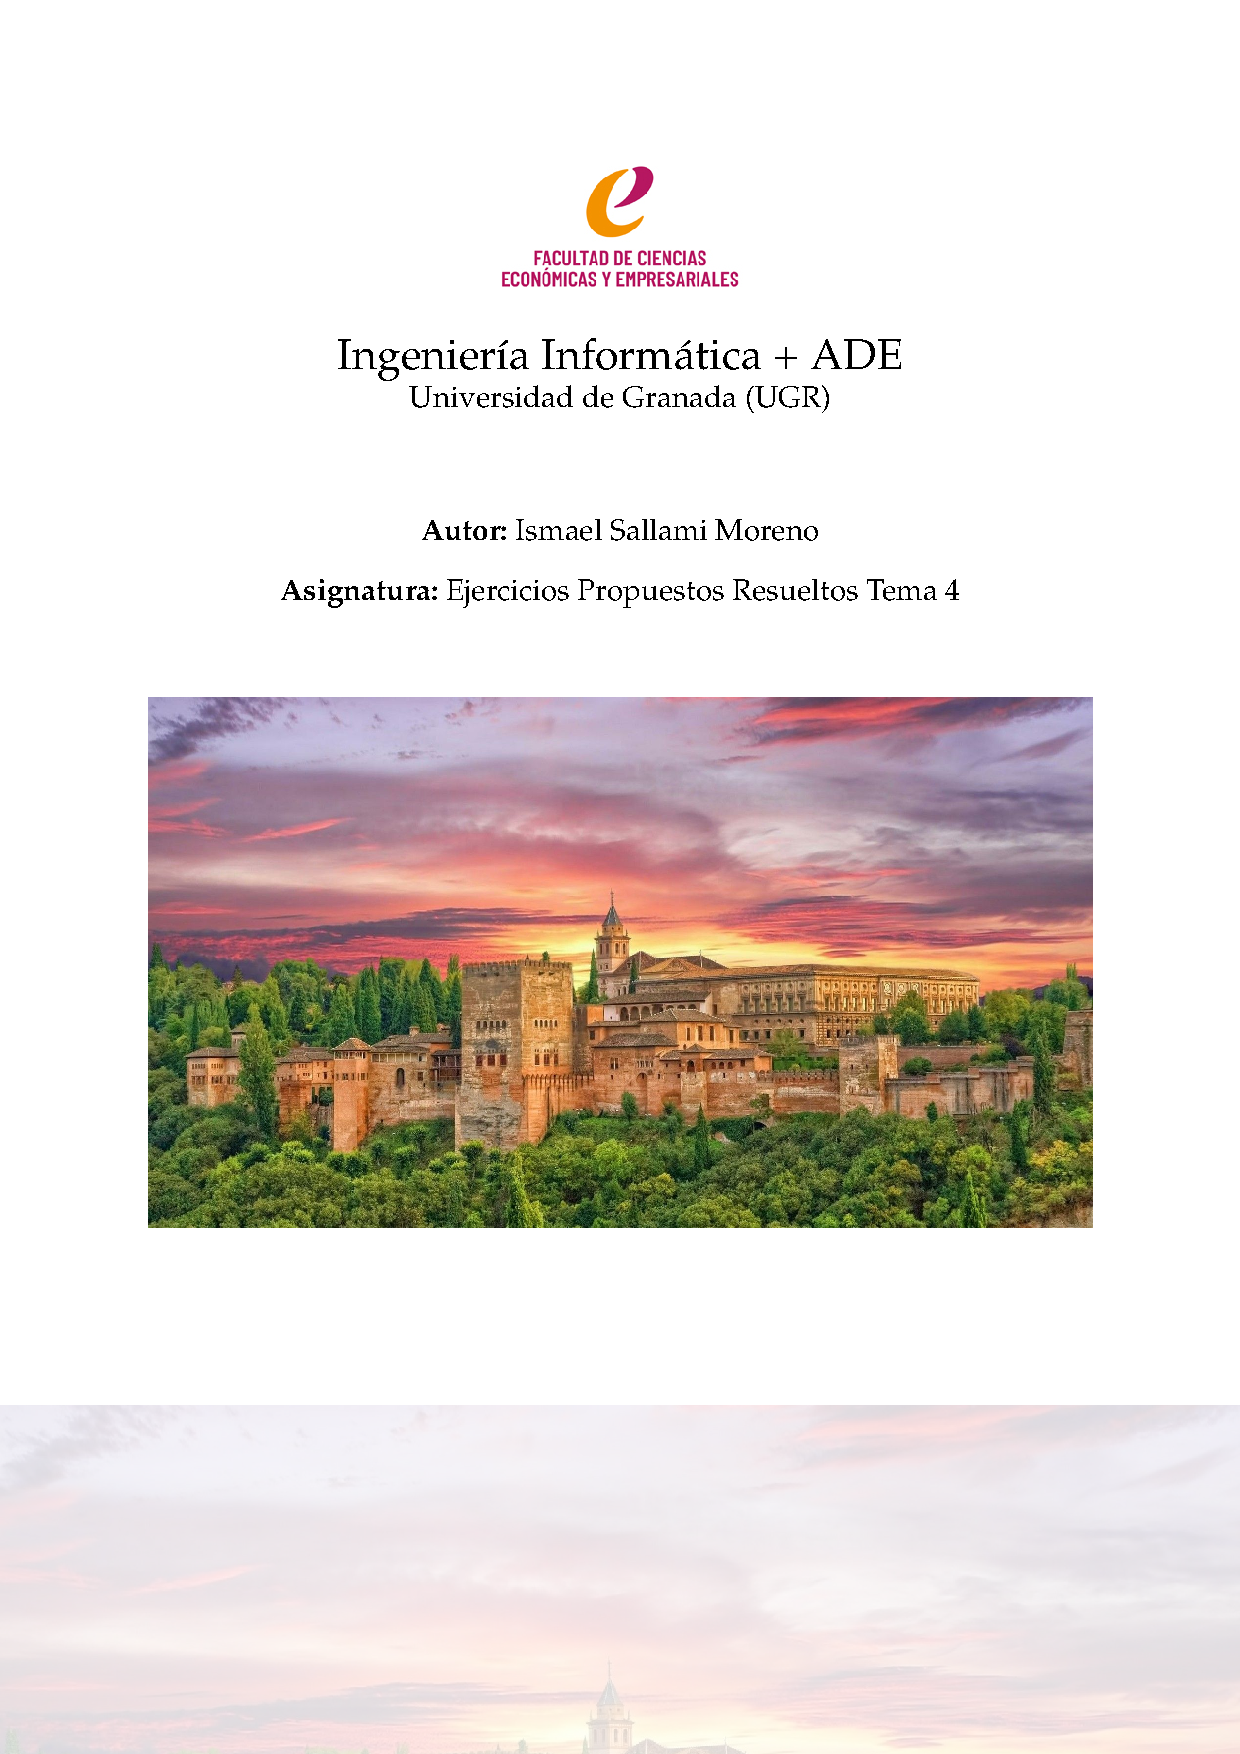
\includepdf[pages=-]{../Tema4/EjerciciosPropuestos/FCCEE/build/EjPropT4.pdf}
\subsection{Tema 5}
\includepdf[pages=-]{../Tema5/EjerciciosPropuestos/FCCEE/build/EjerciciosPropuestosT5.pdf}
\subsection{Tema 6}

\includepdf[pages=-]{../Tema6/EjerciciosPropuestos/FCCEE/build/EjerciciosPropuestost6.pdf}

\section{Fuentes de la Información}
\begin{itemize}
    \item Libro de Prácticas: \url{https://www.wuolah.com/}
\end{itemize}

\end{document}
